\section{Workflow}
The overall workflow is  Figure \ref{fig:teaser}

In this section, we shortly walk through the pipeline in our workflow and describe three steps: Digital Model Acquisition, the Game System, and Fabrication. Our system takes textured mesh model or point cloud with colored vertices. As complete mesh model provides more robust result with 3D shapes of branches, we describe our process based on mesh model as input (see Figure \ref{fig:pipeline} ).

\begin{figure}[ht]
  \begin{center}
    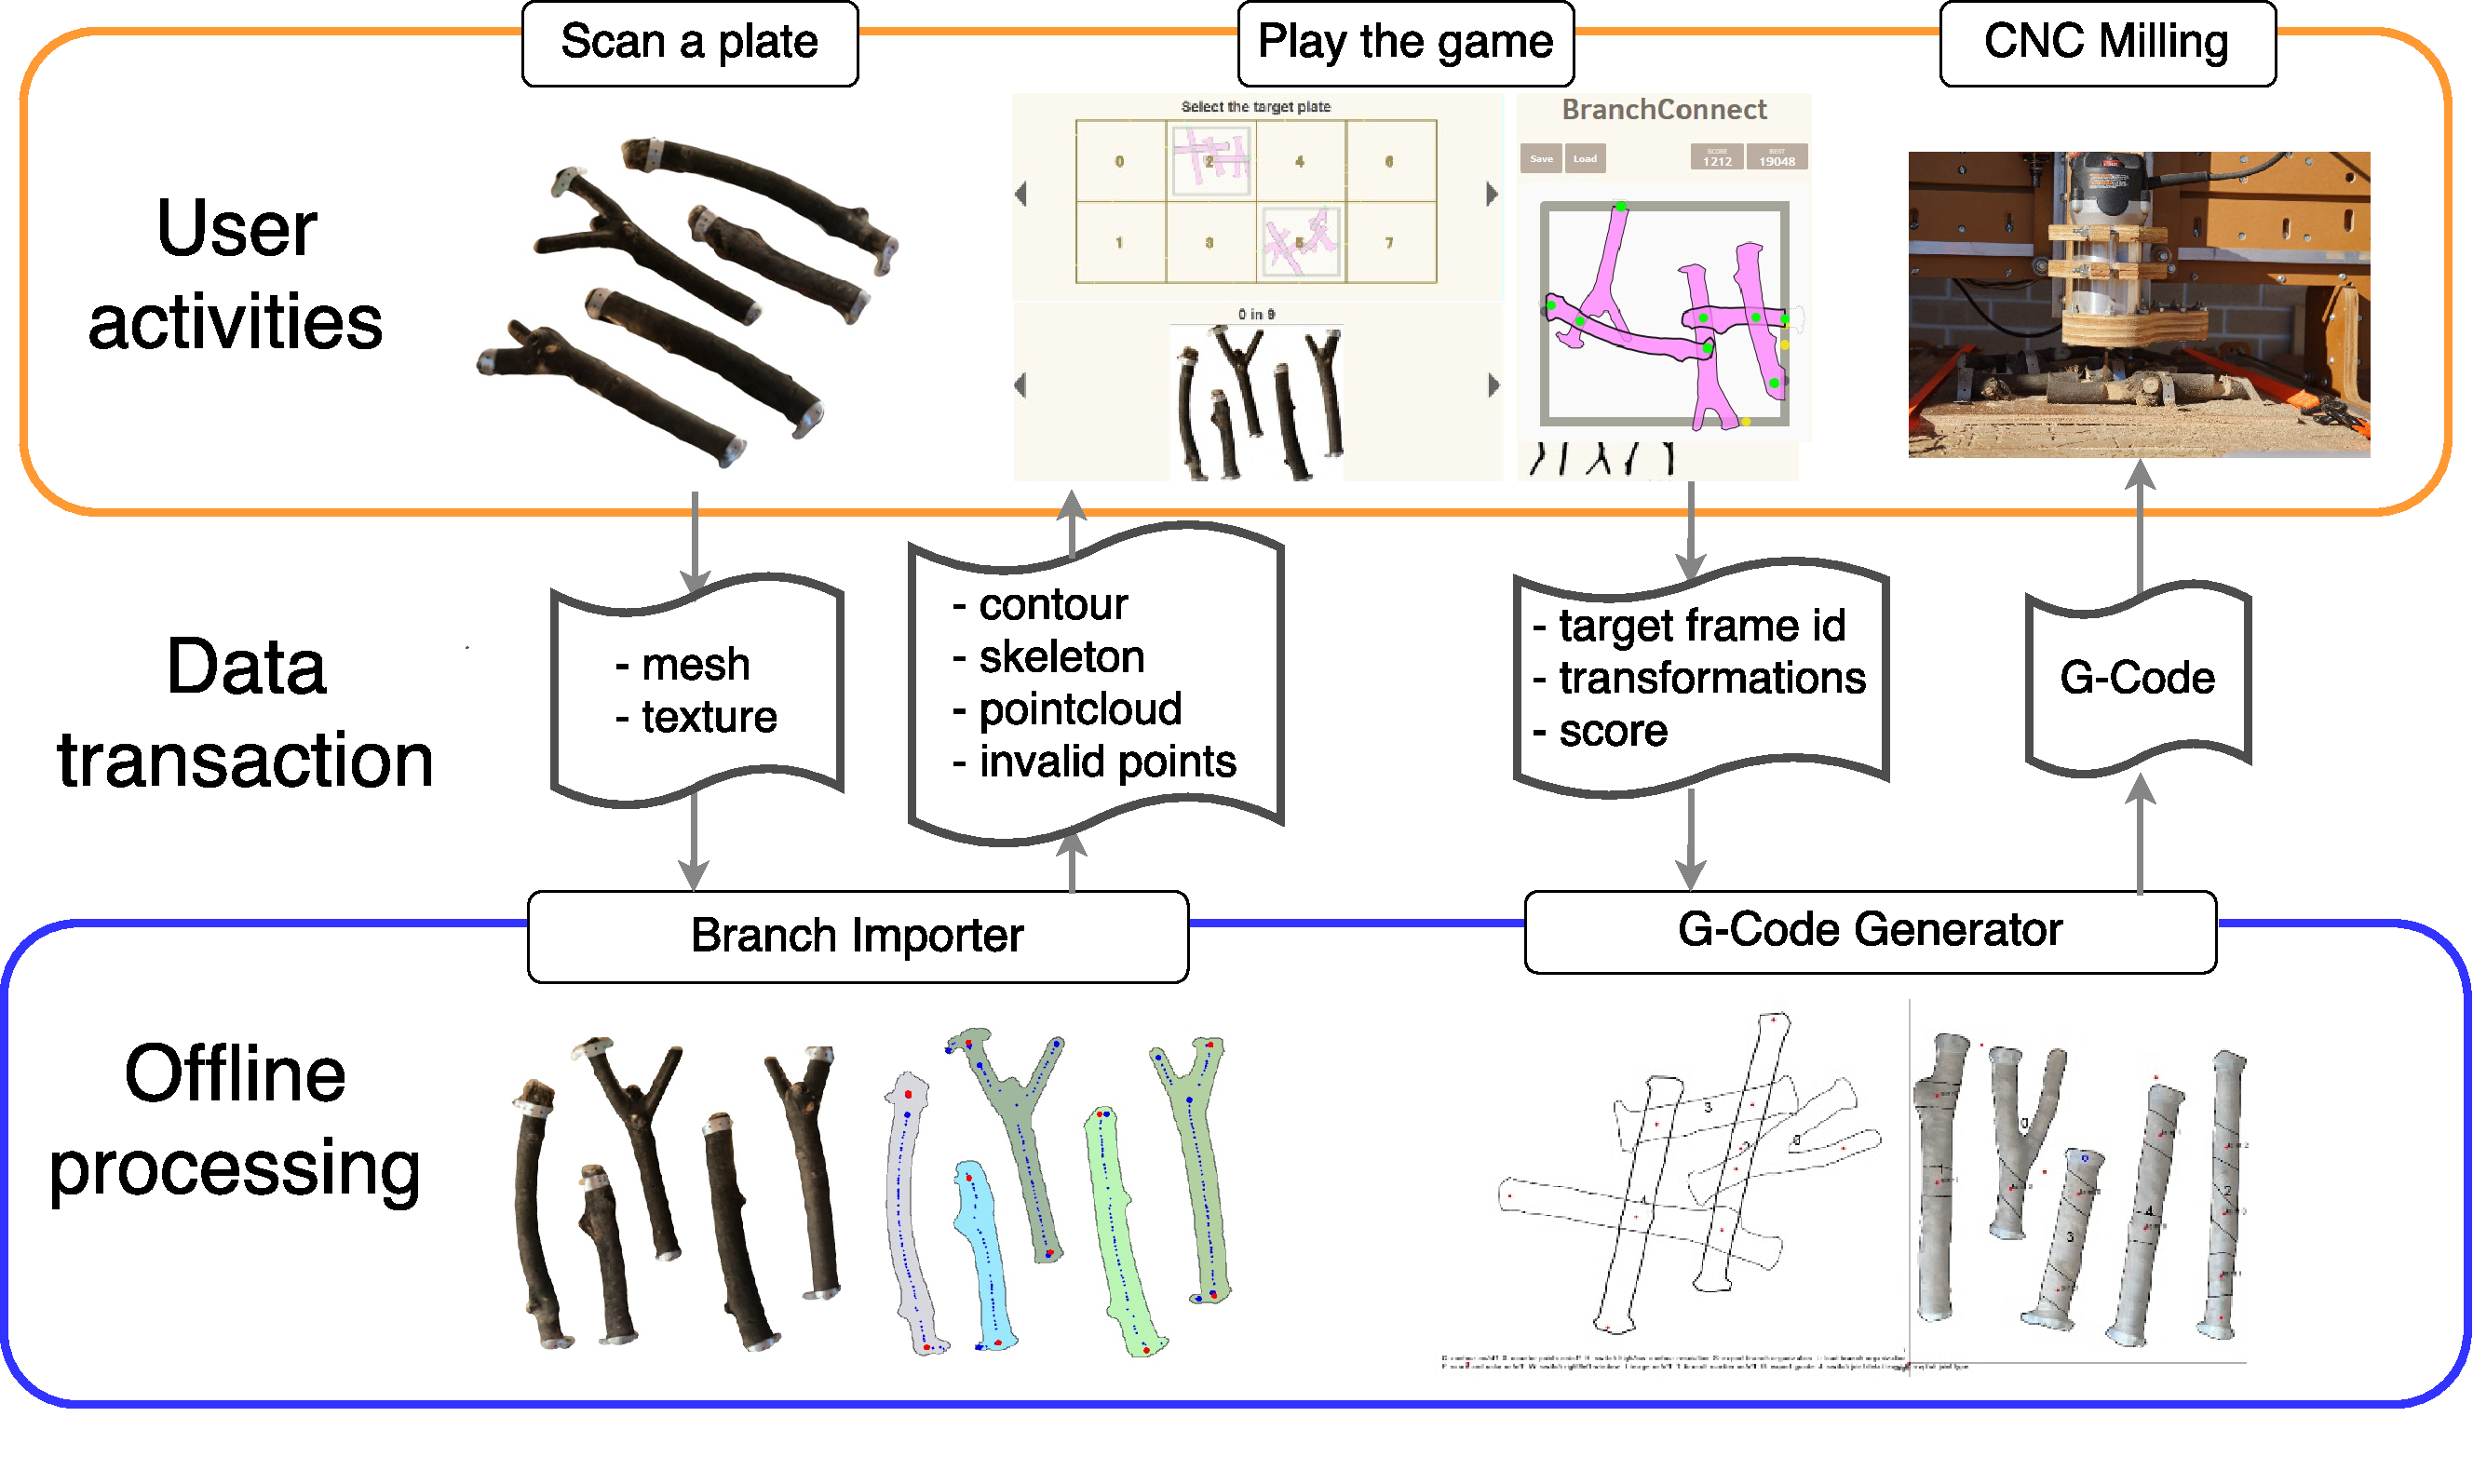
\includegraphics[width = 0.4\paperwidth]{images/workflow/pipeline.pdf}
    \caption{A pipeline from model acquisition to fabrication.}
    \label{fig:pipeline}
  \end{center}
\end{figure}

\subsection{Digital Model Acquisition}
There are various methods and software available for scanning 3D models and detecting objects.
As for the scanning, we describe in the Experiment.
Taking mesh model with colored texture, our \textit{Branch Importer}, integrates necessary functions such as object detection, skeleton extraction, branch type classification, and fixture location detection.

% The acquired model is segmented from the attached plate by a height threshold value.

After segmenting branches from a plate by height threshold, each branch is detected using \textit{findContour} in OpenCV \footnote{Open Source Computer Vision Library. See \url{http://opencv.org/} }.
The obtained 2D contours are used for extracting skeletons and clustering point cloud in the mesh model.
Contours are triangulated and skeleton points are extracted from middle points on edges of triangles.
These middle points are compared with binary top view image of the mesh model (contours are filled with different colors and the background is white).
If the point is inside of a contour, the middle point is counted in skeleton points.
Metal fixture locations are also filtered out due as they have bright reflections on original images, however, we also double check with simple mouse-clicks to ensure these invalid points.
After extracting valid middle points, connectivity of skeletons is analyzed by angle of three adjacent skeleton points.
If the angle stays within a threshold bound, a point is counted in a sub-branch, otherwise, new sub-branch is created.
Evaluating the number of sub-branches, the branch is morphologically classified.
Most branches are categoraized in three shapes:  $I, V, and Y$ shapes.
$I$ shape has a straight continuous polyline, $V$ has an inflection point, and $Y$ has a splitting point.
The acquired information is stored in a cloud database.

\begin{figure}[ht]
  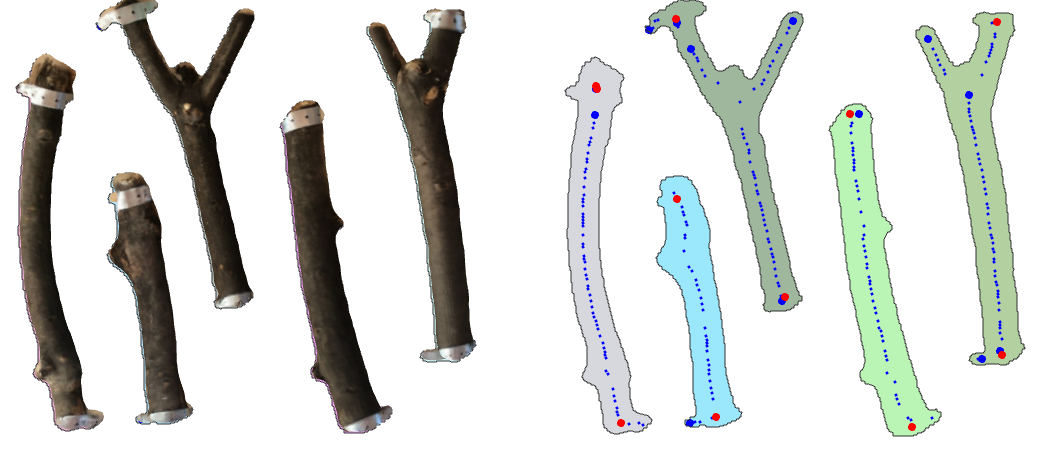
\includegraphics[width = 0.4\paperwidth]{images/importer/importer.png}
  \caption{An overview of \textit{Branch Importer}. Left: a top ortho-view image of textured mesh model. Right: Extracted skeletons (blue dots). The beginning of skeletons is shown bigger dots. Red dots are invalid points. }
  \label{fig:skeleton}
\end{figure}




\subsection{BranchConnect: The Game}
The game objective is to collect valid compositions of branches which structurally sounding and possible to fabricate with ordinal 3 axis CNC milling machines.
The workflow of the game is illustrated in Figure~\ref{fig:game_flowchart}

\begin{figure}[ht]
  \begin{center}
    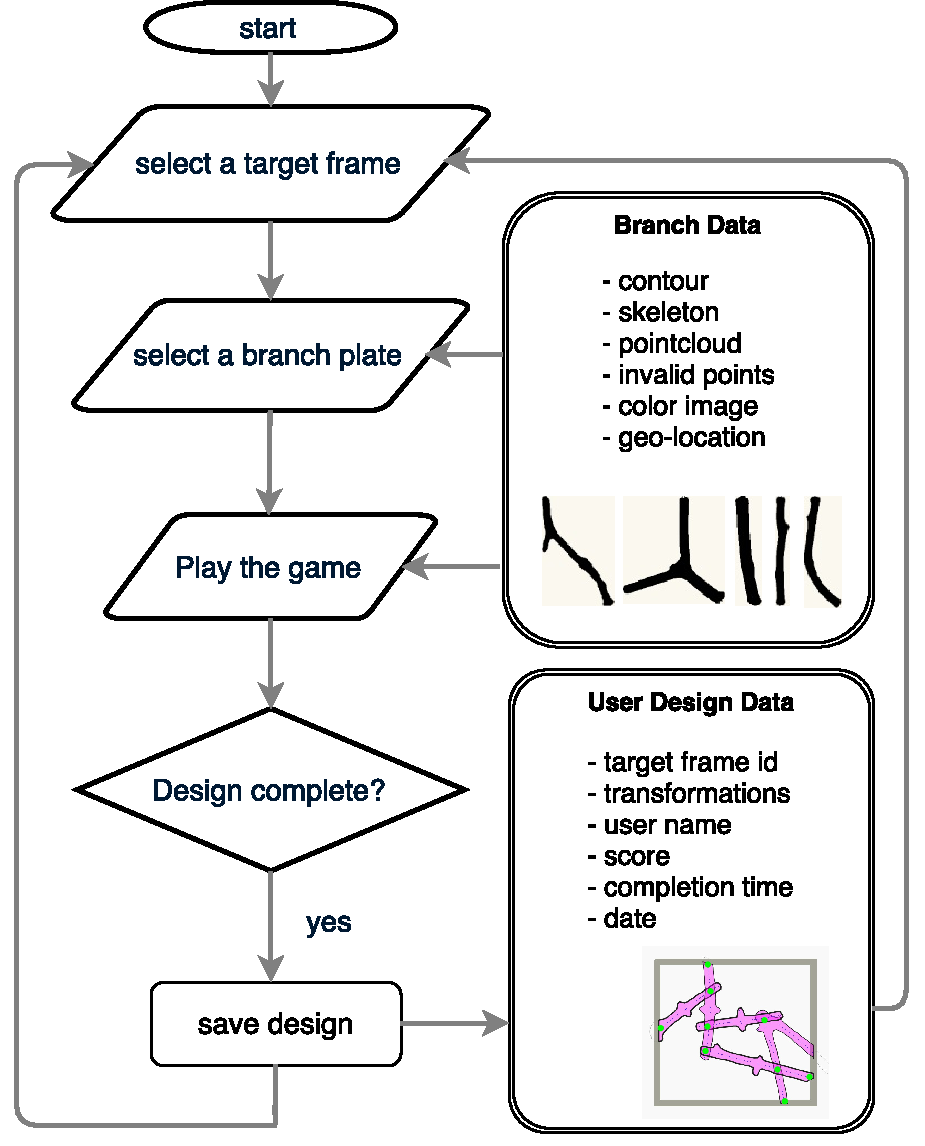
\includegraphics[width = 0.25\paperwidth]{images/system/systemFlowChart.pdf}
    \caption{The workflow of \textit{BranchConnect}. Branch data and user design data are stored on cloud database.}
    \label{fig:game_flowchart}
  \end{center}
\end{figure}

Firstly a user selects a frame indicating multiple target points to be connected, and then selects a set of branches fixed on a plate (The left in Figure \ref{fig:game_interface} ).
After selecting the target frame and the set of branches, the user is guided to the game interface, consisting of the frame with the target points, and the set of available branches (The right in Figure \ref{fig:game_interface} ).
The user picks a branch from the available set on the bottom, and then places it in an arbitrary 2D pose through basic manipulations such as move, rotate, and mirror.
The number of available branches differs depending on plates.
With the feasible diameter of branches (over 2cm) and the plate size (50cm x 50cm), the number of available branches is most likely up to six.
Within the limited number of branches, the user bridges all the target points by connecting all the used branches in one group.
The game is completed when all the target points are connected by branches.
For higher score, the user can modify the design after the completion.
After completing the modification, the design is submitted and sent to \textit{G-Code Generator}.

\begin{figure}[H]
  \begin{center}
    
\includegraphics[width = 0.4\paperwidth]{images/interface/game_interface.png}
    \caption{Left: the selection interface for target frames (top) and branch panels (bottom). Right: the start interface of the game.}
    \label{fig:game_interface}
  \end{center}
\end{figure}
%
\subsubsection*{System Overview}
There are many collision detection libraries available, however, our game needs to detect intersected branch pairs, thus surface contact detection is overkill for our application.
Also most branches come with free-form concave shapes, thus further geometric preparation such as convex decomposition is necessary for using these libraries.
For fast and robust intersection detection, our system extensively uses skeletons of branches.
Hubbard and Philip developed collision detection by representing object with hierarchical 3D spheres aligned on skeletons \cite{Hubbard:1996:APS:231731.231732}.
Our system takes similar approach but more limited in 2D and intersection detection only.
In broader phase, simplified skeletons are used to find the pair of closest skeleton points between two branches.
After finding the pair, skeletons with higher resolutions are used.

A joint is created when an intersecting pair is detected, and the pair forms a group.
The group is used for evaluating connections between target points.
The game is completed once all the target points are connected by a group of branches.
The conditions of joint and group are indicated with simple color-code.
Once the user finishes positioning, score is updated with weighted sum of parameters.
Together with the color-code, the score update guides the user to form a valid design.
An overview is illustrated in Figure \ref{fig:system_flowchart}.

\begin{figure}[ht]
  \begin{center}
    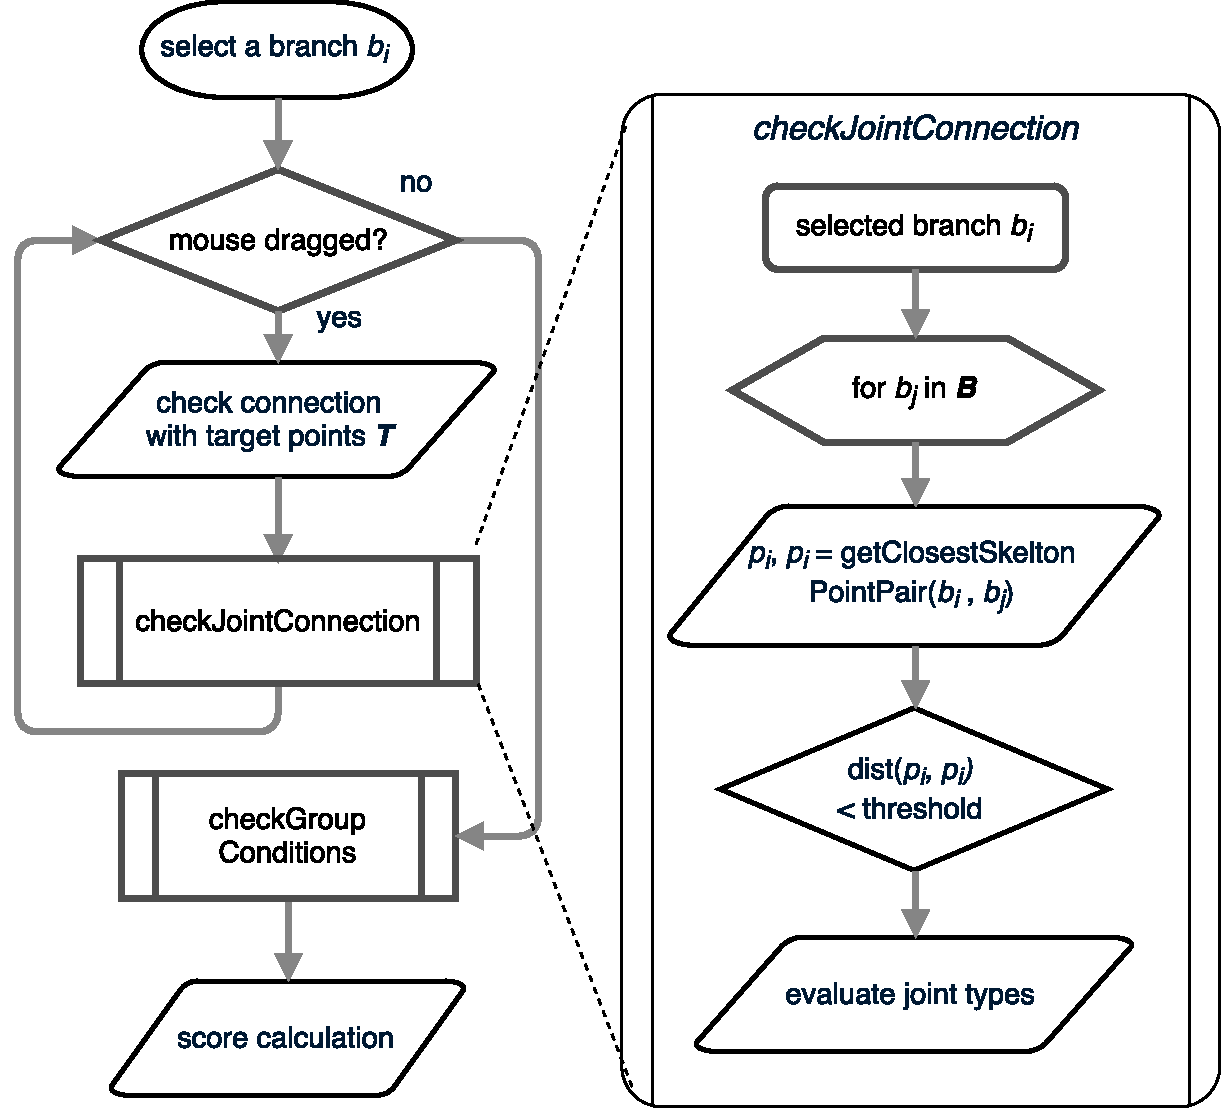
\includegraphics[width = 0.25\paperwidth]{images/system/closestPointAlgorithm.pdf}
    \caption{Left: an overview of the game system. Right:joint condition checking process.}
    \label{fig:system_flowchart}
  \end{center}
\end{figure}

\subsubsection*{Joint Condition}
Joint is the essential entity not only in the game but also the entire project including the fabrication process.
The closest skeleton point pair is obtained
We accept crossing joints only because they are structurally stable, relatively simple to fabricate, and creates diverse designs.
To ensure the structural performance, we set a connection angle within a range from 45 to 135 degrees.
Joints close to metal fixtures are also counted as invalid.
Valid and invalid joints are displayed with green and red respectively.
The color-code feedback is also given when target points on a frame is connected with a branch.
Figure~\ref{fig:joint_condition} illustrates valid and invalid joint conditions.


To describe the process, we let $\mathcal{B}$ denotes a set of all the available branches, and each branch as $ b_i \in \mathcal{B}$.
While the process checks joint condition through all the branches $\mathcal{B}$, each detected joint is stored in each branch $b_i$, categorized in different conditions such as valid and invalid joints denoted as
$\mathcal{J}_{\text{valid},i}$,
$\mathcal{J}_{\text{invalid},i}$ respectively, together with the paired branch id $b_{\text{paired},j, i}$.
When a branch is connected to one of target point $t_j \in \mathcal{T} $, the $t_j$ is stored in $p_i$ as $t_{j,i}$.
\todo{notaion should be improved!}

% well as the paired branch $b_{\text{paired},j} \in \mathcal{P}_{\text{paired},i}}$.

\begin{figure}[ht]
  \begin{center}
    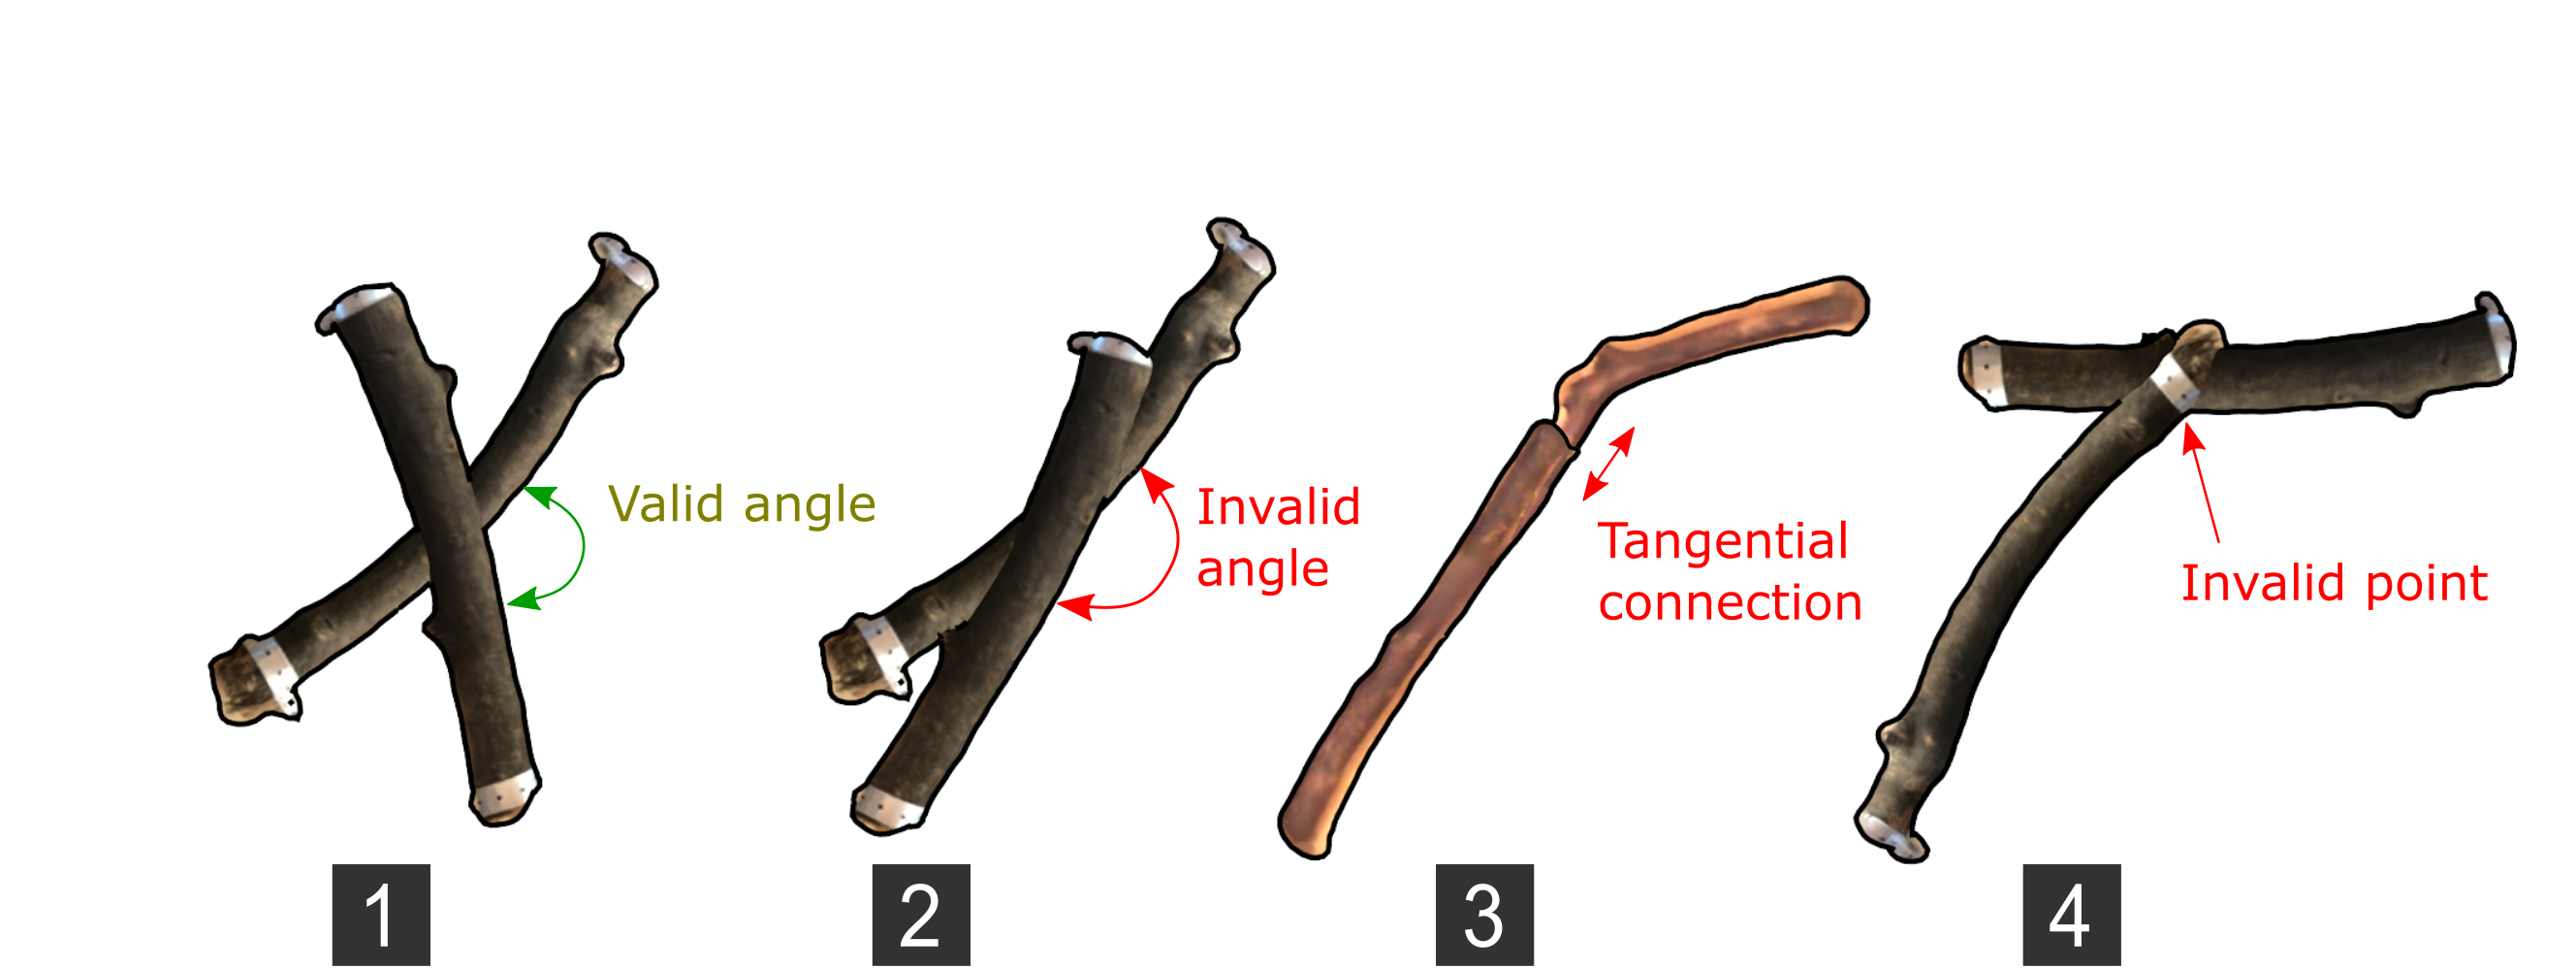
\includegraphics[width = 0.4\paperwidth]{images/system/joint_conditions_2.png}
    \caption{Joint conditions. 1.valid joint. 2.invalid for violating the angle. 3.invalid tangential connection. 4.invalid for connecting on a fixture point. }
    \label{fig:joint_condition}
  \end{center}
\end{figure}

\subsubsection*{Group Condition}

After checking joint conditions of all the pairs of branches, the system checks the number of groups as well as connectivity with the target points on a frame.
If a group is not connected to any target point nor other groups, the group is islanded and structurally invalid.
While a user is positioning a branch by dragging or rotating, groups are continuously calculated and indicated by simple color (Figure \ref{fig:group}).

\begin{figure}[ht]
  \begin{center}
    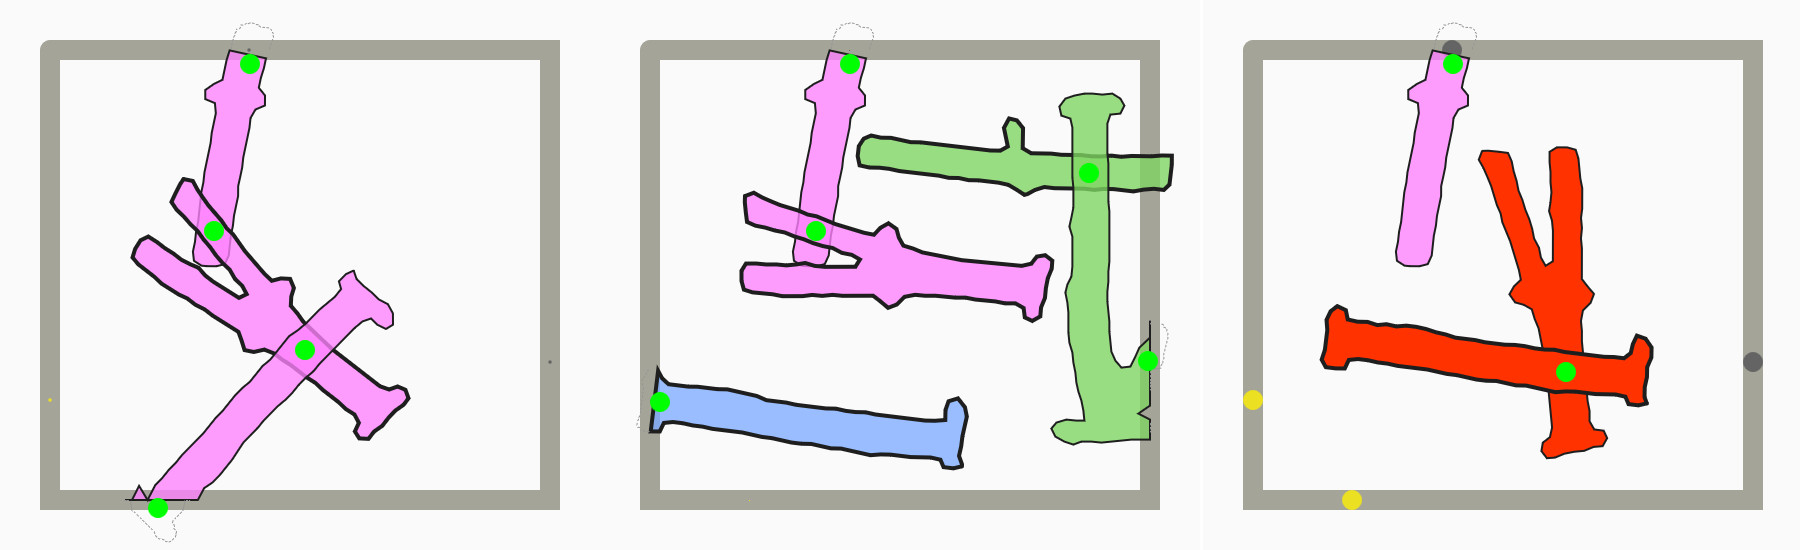
\includegraphics[width = 0.4\paperwidth]{images/interface/groups.jpg}
    \caption{Left: valid group with two target points connected. Middle: valid but three groups. Right: invalid due to the island situation. }
    \label{fig:group}
  \end{center}
\end{figure}


After all the joint conditions are checked, we evaluate group conditions.
Through checking the all the branches $\mathcal{B}$, the first group $g_0$ is created and stores $b_0$.
The other paired branch $b_{\text{paired},i}$ is used to trace the connection with other  compared to the  traced through the stored paired branch  in each valid joint $j_i$.
 in all groups $\mathcal{G}$.
The game is completed when the number of $\mathcal{G}$ is one, and all the target points are connected with the group.

\begin{algorithm}
  \caption{Group Condition Update Algorithm}
  \begin{algorithmic}[1]
    \Function{UpdateGroups}{$\mathcal{B}$}
    \State{Reset all the groups $\mathcal{G}$ }
    \State{Create new group $g_1$}
    \State{$g_1 \text{ add } b_1$}
    \If{$b_1$ has connected target point $t_1$}
      \State{$g_1 \text{ set } t_1$}
    \EndIf
    \State{$\mathcal{G} \text{ add } g_1$}

    \For{each branch $b_i$ in $\mathcal{B}$}
    \State{\textit{GroupConnection} $\gets false$}
      \For{each group $g_j$ in $\mathcal{G}$}
        \For{each branch $b_j$ in $g_j$}
          \If{ $b_{\text{paired},i} \in \mathcal{P_i}$ has $b_j$}
            \State{ $g_j \text{ add } b_i$}
            \State{ \textit{GroupConnection}  $\gets true$}
            \If{($b_i$ has $t_i$) and ($g_j$ has $t_j$) }
              \State{ Set $g_j$ as \textit{Bridged}}
            \EndIf
            \If{$g_j$ has no $t_j$}
              \State{ Set $g_j$ as \textit{Islanded}}
            \EndIf
            \State {\textit{break}}
          \EndIf
        \EndFor
      \EndFor

      \If{ \textit{GroupConnection} is \textit{false} }
        \State{create new group $g_{new}$}
        \State{ $g_{new} \text{ add } b_i$}
        \State{$\mathcal{G} \text{ add } g_{new}$}
      \EndIf
    \EndFor

  \EndFunction
  \end{algorithmic}
  \label{al:connection}
\end{algorithm}

\subsubsection*{Score Calculation}
We denote the numbers of valid and invalid joints on each branch $b_i \in \mathcal{B}$ as $N(valid_i)$ , $N(invalid_i)$ respectively, the number of groups as $N(\mathcal{G} )$, the number of islanded groups as $N(g_{\text{islanded}} \in \mathcal{G} )$, the number of bridged target points as $N(t_{\text{bridged}, i}) \in \mathcal{T} )$.
The score is weighted sum of these joint and group conditions (see Eq \ref{eq:cost}).

\todo{notaion should be improved!}
\begin{equation} \label{eq:cost}
 \begin{aligned}
 Score =  &\; w_1  \sum_{1}^{N(\mathcal{B})}N(valid_i) \; +
\; w_2  \sum_{1}^{N(\mathcal{B})} N(invalid_i) \\
+ &\; w_3  \sum_{1}^{N(\mathcal{G})} g_{\text{islanded}} \;+
\; w_4  \sum_{1}^{N(\mathcal{T})} t_{\text{bridged}}
 \\
   \textrm{s.t.} \; w_j  \geq  &\;0 \; \forall j \in 1, \dotsc , 4
 \end{aligned}
\end{equation}

\subsection{Fabrication}
After a design is selected for fabrication, the validity of the design is further inspected with a high-resolution model.
The \textit{G-Code Generator} was developed for fine-tuning the design by checking real-time feedback of updated joineries on branches with scanned orientations (see Figure \ref{fig:gcode_gen}).

\begin{figure}[ht]
  \begin{center}
    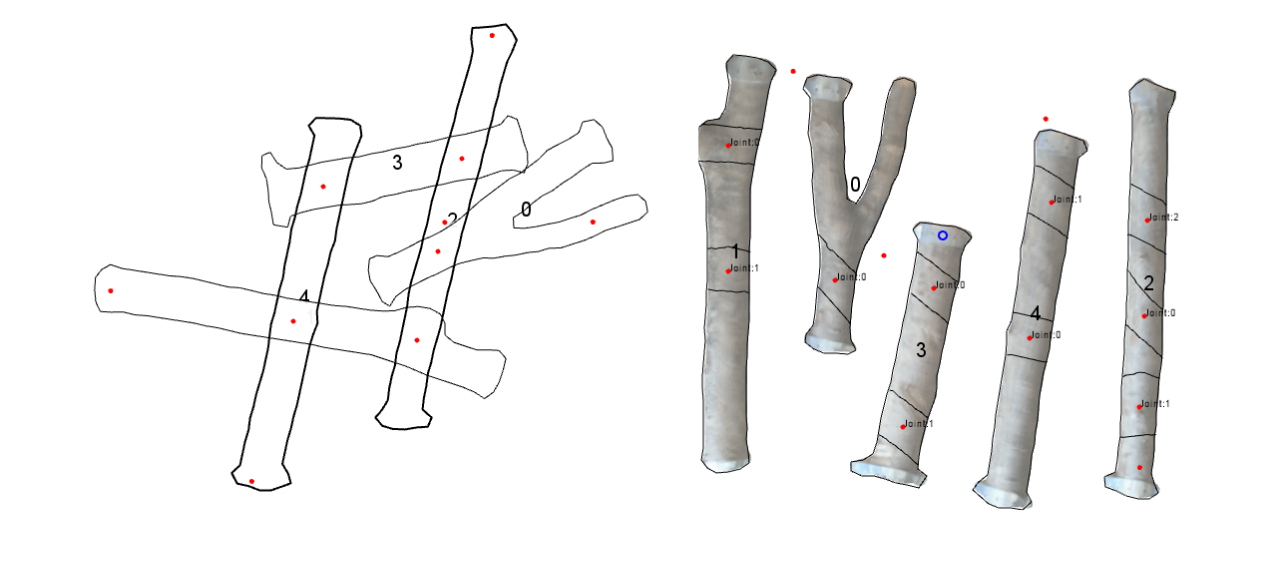
\includegraphics[width = 0.4\paperwidth]{images/system/joint_generator_2.png}
    \caption{Interface of \textit{G-Code Generator}. Users can tweak the design on the left side and immediately see the updated joints and milling paths on the right. \todo{can this image be integrated with the other one?}}
    \label{fig:gcode_gen}
  \end{center}
\end{figure}

Some fabrication factors such as mirror and invalid points are already considered by \textit{Branch Importer} and the game system of \textit{BranchConnect}.
In this section, we describe the process of joinery generation.
Each joinery geometry is different but has same topology: two plane surfaces on the sides of branches and one plane top surface.
The geometry creates rigid connection with the irregularly shaped sections of branches.
Similar to the joint searching process with skeletons, the \textit{G-Code Generator} searches a set of four closest points from high-resolution contours, expecting that every intersected contour has four curves.
After finding the four closest points, it trims two curves from each contour of branch. (two from intersecting branch and two from intersected branch) at each joint.
The trimmed contours are transformed to the original scanned orientation and used for generating milling paths.
Two curves from an intersected branch are used for side cuts milling paths, which are inwardly offset paths of the original branch contours. \todo{need to brush up!}
The center cuts are paths that are plaining the top surface of the joint.
\todo{describe the cutting height calculation!}

\begin{figure}[ht]
  \begin{center}
    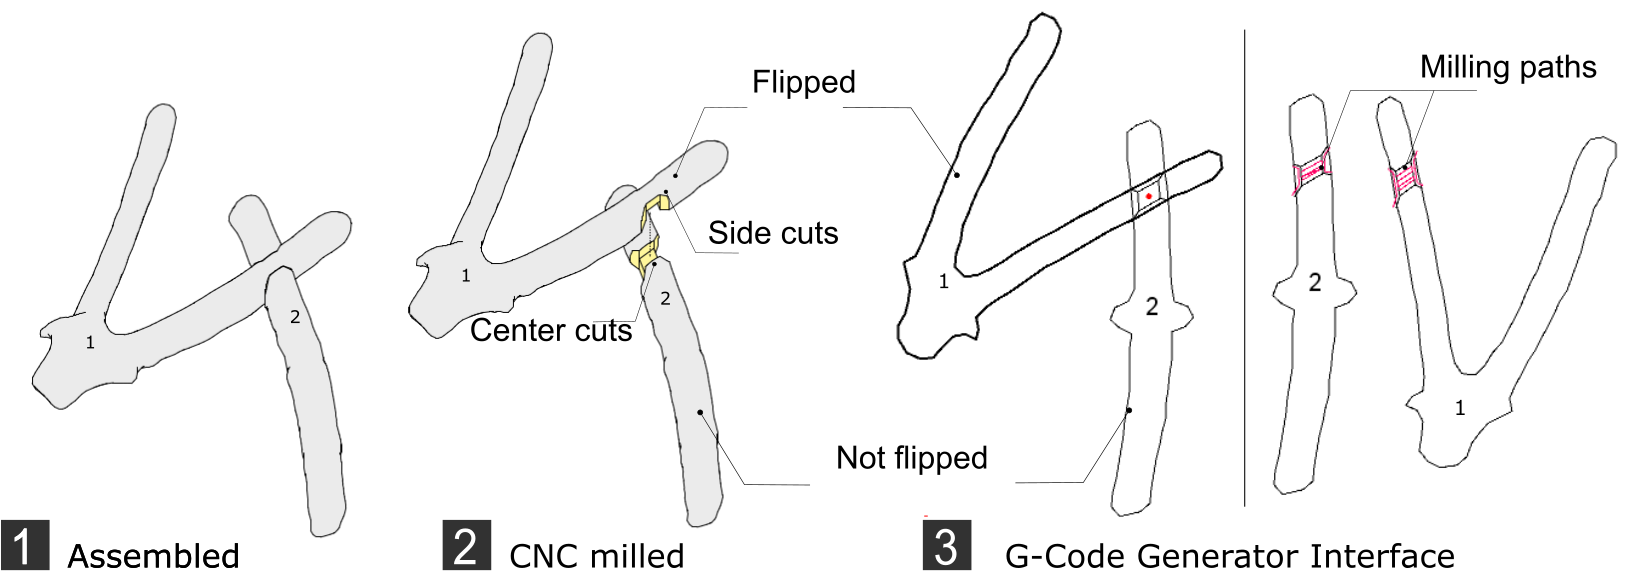
\includegraphics[width = 0.4\paperwidth]{images/system/joint_milling_diagram_4.png}
    \caption{An example of intersected pair: 1. an assembled pair of branches. 2. branches after the center and side cuts are milled 3. left: a composition defined by a user right: the original orientations of branches with generated milling paths with red color.  }
    \label{fig:joint_geometry}
  \end{center}
\end{figure}

Users can change fabrication parameters such as offset ratio for the side cuts, milling bit diameter, overlapping ratio for defining the center cut depth, feed-rate, moving height and so forth.
After confirming the fabrication settings and milling paths, it generates G-Code.
